% \documentclass[aps,prb,superscriptaddress,showpacs,amsmath,amssymb,letterpaper]{revtex4}
% \usepackage{graphicx}
% \usepackage{epsfig,color,verbatim} % multi-line comments
% \usepackage{subfigure}             % allows for use of "sub figure" 1a, 1b, etc
% \usepackage{hyperref}

%\begin{document}

\chapter{Relation between transmission and energy stored in random media with gain}
\label{chap:TE_gain}
\label{paper:1_start}

% \author{Ben Payne$^{1}$, Jonathan Andreasen$^{2}$, Hui Cao$^{2}$, and Alexey Yamilov$^{1}$\footnote{Email: yamilov@mst.edu}\\
\begin{center}
Ben Payne$^1$, Jonathan Andreasen$^2$, Hui Cao$^2$, and Alexey Yamilov$^1$      \label{sec:TE2009}                                                                         \end{center}

\ \\
\begin{center}
\textit{$^1$Department of Physics, Missouri University of Science \& Technology,\\ Rolla, MO 65409\\
$^2$Department of Applied Physics, Yale University, New Haven, CT 06520}\end{center}

\ \\
% {\it $^{1}$Department of Physics, Missouri University of Science \& Technology, Rolla, MO 65409\\
% $^{2}$Department of Applied Physics, Yale University, New Haven, CT 06520}}
% \noaffiliation
% \date{\today}
% \begin{abstract}
\addcontentsline{toc}{section}{ABSTRACT}
\begin{center}\textbf{ABSTRACT\footnote{Published in Physical Review B \textbf{82} 104204 (2010).}}        \end{center}

In this work, we investigate a possibility of using the ratio between optical transmission, $T$, and energy stored inside the system, ${\cal E}$, as a quantitative measure of the enhanced mesoscopic corrections to diffusive transport of light through a random medium with gain. We obtain an expression for $T/{\cal E}$ as a function of amplification strength in the diffusive approximation and show that it does not a have tendency to diverge when the threshold for random lasing is approached, as both $T$ and ${\cal E}$ do. Furthermore, we find that a change in $T/{\cal E}$ signifies a change in the electric field distribution inside the random medium. In the localization regime, we also investigate the correlations between transmission and energy stored in the medium with and without amplification. Our results suggest that $T/{\cal E}$ is a promising parameter which can help characterize the nature of wave transport in random medium with gain.
% \pacs{42.25.Dd,42.55.Zz,72.15.Rn}
% \end{abstract}
% \maketitle 

%\tableofcontents

%%%%%%%%%%%%%%%%%%%%%%%%%%%%%%%%%%%%%%%%%%%%%%%%%%%%%%%%%
\section{INTRODUCTION}
\label{sec:intro}
%%%%%%%%%%%%%%%%%%%%%%%%%%%%%%%%%%%%%%%%%%%%%%%%%%%%%%%%%

Anderson localization \cite{1958_Anderson} (AL) is a wave phenomenon \cite{1960_Ioffe_criterion,1984_John_prl,1985_Anderson} that leads to a breakdown of diffusion\cite{1980_Vollhardt_Wolfle,1991_Altshuler}. First conceived in electronic systems, it originates from  a repeated self-interference of de Broglie waves during their propagation in a random potential. Conservation of number of carriers, enforced because the electrons possess an electric charge, lies in the foundation of the concept of AL. 

Understanding the effect of absorption \cite{1984_John_prl}, ubiquitous in optical systems, turned out to be essential for proper physical description and interpretation of experimental studies of {\it light} localization \cite{1989_Genack,1997_wiersma_nature,1999_Maret,2000_chabanov_nature,2007_Maret,2007_Segev}. It also prompted the search\cite{2000_chabanov_nature} for an alternative criterion of localization in absorbing media. Coherent amplification, which leads to an altogether new physical phenomenon of random lasing\cite{2005_Cao}, demands further refinement of the concept of AL and its criteria in active random media.

In the case of absorption, an alternative criterion, based on the magnitude of {\it fluctuations} of transmission normalized by its average, was put forward \cite{2000_chabanov_nature}. In random media with gain, this quantity (as well as any other statistically averaged quantity) becomes ill-defined \cite{2005_Yamilov_correlations}. This is because there always exists a non-zero probability of encountering a special realization of disorder within the statistical ensemble where the given value of the gain parameter exceeds the threshold for random lasing\cite{2005_Cao}. Without saturation effects, such a realization will have an infinite contribution to a statistical average. Inclusion of the saturation introduces a dependence on system- and material-specific parameters which are not associated with wave-transport properties of the random medium. To avoid such dependence, and at the same time to regularize the statistical ensemble, in Ref. \cite{2005_Yamilov_correlations} we introduced conditional statistics by excluding the diverging contributions. Such an approach indeed turned out to be fruitful in studies of enhanced fluctuations and  correlations in mesoscopic transport of the electromagnetic waves through random medium with optical amplification \cite{2004_Yamilov_intensity,2005_Yamilov_correlations,2006_Yamilov_conductance}. These investigations also motivated us to explore an intriguing possibility of localization by gain -- enhancement of the mesoscopic phenomena with an increase of the amplification strength.

In this work, we investigate the properties of the ratio between transmission $T$ and the energy inside a random medium ${\cal E}$, with the goal of formulating a criterion of AL which would be applicable in the presence of gain. Both parameters should be experimentally accessible in planar systems, e.g. perforated dielectric films, in which the spatial field distribution inside the medium can be obtained via near-field scanning optical microscopy.

In Section~\ref{sec:diffusion_section}, to motivate our choice of the parameter in the form $T/{\cal E}$, we consider random medium in regime of diffusive transport. First we note that when taken separately, both transmission and the energy inside the system ${\cal E}$ exhibit an expected tendency to increase with an increase of the gain strength and to diverge when threshold for random lasing is approached (no saturation mechanism is assumed). However, when taken in a form of a ratio, the divergence is eliminated and the tendency to increase is greatly reduced. Secondly, we show that in passive systems the ratio can be related to the spatially-dependent diffusion constant $D(z)$. The latter concept has been recently invoked \cite{2008_Cherroret,2010_Payne_PRL} in the self-consistent theory of AL to extend the applicability of diffusion approximation into the localized regime. The connection between $T/{\cal E}$ and $D(z)$ demonstrates that the former can, indeed, be used as  a quantitative measure of the contribution of localization (interference) phenomena in transport through disordered systems.

In Section~\ref{sec:diffusion_general} we obtain an expression for $T/{\cal E}$ from the solution of the diffusion equation in a random medium (using the slab geometry) with gain. This establishes a baseline -- a decrease of the parameter $T/{\cal E}$ below the diffusion prediction obtained in this section can be used to quantify the extent to which the gain promotes the localization effects.

In order to further assess the usefulness of $T/{\cal E}$ as a localization criterion, in Sec.~\ref{sec:localization_passive} we also consider random medium in the localized regime where we investigate the correlations between the transmission and stored energy in the same disorder configuration. We show that the ratio strongly depends on the spatial location of localization center. This introduces an additional (geometrical) source of fluctuation which is not present in the transmission coefficient alone. Interestingly, this effect leads to profound gain-induced modification of the electric field distribution inside the system that is studied in Sec.~\ref{sec:localization_gain}. 

Discussion of the obtained results and an outlook is given in Sec.~\ref{sec:discussion_TE}.

%%%%%%%%%%%%%%%%%%%%%%%%%%%%%%%%%%%%%%%%%%%%%%%%%%%%%%%%%
\section{ANALYSIS OF \texorpdfstring{$T/{\cal E}$}{T/E}: DIFFUSIVE REGIME}
\label{sec:diffusion_section}
%%%%%%%%%%%%%%%%%%%%%%%%%%%%%%%%%%%%%%%%%%%%%%%%%%%%%%%%%

\subsection{Model Description}
\label{sec:diffusion_eq}

In weakly scattering random media it is common to disregard the wave nature of carriers (electrons, photons, etc) and to describe the transport in terms of the phase-less diffusion equation. Under this condition, the ensemble-averaged diffusive flux $\langle{\bf J}({\bf r},t)\rangle$ and the energy density $\langle {\cal W}({\bf r},t)\rangle$ are related via\cite{1953_Morse}
\begin{equation}
\langle{\bf J}({\bf r},t)\rangle=-D({\bf r})\boldnabla\langle {\cal W}({\bf r},t)\rangle.
\label{eq:Jflux}
\end{equation}
The diffusion approximation amounts to $D({\bf r})\equiv D_0=v_E \ell/3$, where $\ell$ is transport mean free path and $v_E$ is the energy transport velocity \cite{1991_van_Albada_vE}. In the following we will neglect resonant scattering effects and will assume that $v_E$ is equal to the speed of light in vacuum. 

Vollhardt and W\"{o}lfle \cite{1980_Vollhardt_Wolfle} laid out a theory which allows one to account for wave interference effects while retaining diffusive-like formalism. With recent refinements \cite{2008_Cherroret,2010_Payne_PRL}, it is currently believed that allowing for renormalization and spatial dependence of the diffusion coefficient $D({\bf r})$ provides an adequate description of transport through random medium of finite size even beyond the diffusive regime. At the same time, deviation (reduction) of $D({\bf r})$ from the constant value of $D_0$ is interpreted as a manifestation of the developing localization effects.

Eq.~(\ref{eq:Jflux}) has to be complemented by the energy conservation condition
\begin{equation}
\frac{\partial \langle {\cal W}({\bf r},t)\rangle }{\partial t}+{\rm div}\langle{\bf J}({\bf r},t)\rangle=
\frac{c}{l_g}\langle {\cal W}({\bf r},t)\rangle+J_0 \delta(z-z_p),
\label{eq:Jflux_conserv}
\end{equation}
where $l_g$ is gain length and we assume that the coherent flux of an incident plane wave is converted into diffusive flux $J_0$ at $z=z_p\sim\ell$, the penetration depth \cite{1993_Lisyansky_diffusint}, near the left boundary. The above description can be similarly applied to both for the scalar (e.g. acoustic) waves with ${\cal W}({\bf r},t)=\varepsilon({\bf r})\left|d\psi({\bf r},t)/dt\right|^2/(2c^2)+\left|\boldnabla \psi({\bf r},t)\right|^2/2$ and the electromagnetic waves with ${\cal W}({\bf r},t)=\varepsilon({\bf r})\left|{\bf E}({\bf r},t)\right|^2/2+\mu\left|{\bf H}({\bf r},t)\right|^2/2$ \cite{1953_Morse}. In the former case $c/\varepsilon^{1/2}({\bf r})$ has the physical meaning of local propagation speed of the elastic wave field $\psi({\bf r})$ and in the latter, $\varepsilon({\bf r})$ is the dielectric function and ${\bf E}({\bf r},t)$, ${\bf H}({\bf r},t)$ are the electric and magnetic fields. 

Throughout this work we consider the case of linear gain. Such an approximation is justified for values of gain up to the threshold for random lasing when nonlinear and dynamical effects\cite{2005_Cao,2009_Deych_random_laser_theory,2008_Stone,2008_Conti_opals,2009_Frank} become crucial.

We consider a 3D random medium in the shape of a slab of thickness $L$, where we explicitly  separate the coordinate $z$ normal to the slab from the perpendicular component ${\boldrho}$ as ${\bf r}=({\boldrho},z)$. Under a plane-wave illumination at normal incidence, the dependence on ${\boldrho}$ can be neglected. In this case $J_z(z)$ should be understood as the longitudinal component of the flux per unit of cross-sectional area of the slab.  We will also limit our consideration to a continuous wave (CW) regime where the energy density ${\cal W}(z)$ is stationary: $\partial \langle {\cal W}(z)\rangle/\partial t=0$. Under the above assumptions, the boundary conditions 
\begin{equation}
J_z(z=0)=-J_0R,\ \, J_z(z=L)=J_0T
\label{eq:Jflux_bc}
\end{equation}
together with Eqs.~(\ref{eq:Jflux},\ref{eq:Jflux_conserv}) completely specify the problem.

\subsection{Asymptotic Behavior of \texorpdfstring{$T/{\cal E}$}{T/E}: Passive System Limit}
\label{sec:diffusion_zero_gain}

In Appx.~\ref{app:Dz_derivation} we demonstrate that Eqs.~(\ref{eq:Jflux},\ref{eq:Jflux_conserv},\ref{eq:Jflux_bc}) allow one to obtain the following expression for the ratio between $T$ and ${\cal E}$ in the passive limit $1/l_g\rightarrow 0$:
\begin{equation}
\displaystyle\frac{T}{{\cal E}}\simeq
\displaystyle\frac{1}{J_0} \times
\displaystyle\frac{2D_0}{L^2} \times
\left[
\displaystyle\frac{1}{L}\displaystyle\int_{0}^{L}\displaystyle\frac{D_0}{D(z)}dz
\right]^{-1},
\label{eq:TE_vs_D}
\end{equation}
where the energy stored inside the random medium ${\cal E}$ is formally defined as
\begin{equation}
{\cal E}=\int_0^L\langle {\cal W}(z)\rangle dz.
\label{eq:Energy_definition}
\end{equation}
We note that in the process of deriving Eq.~(\ref{eq:TE_vs_D}), terms on the order of $\sim\ell/L\ll 1$ were dropped.

Eq.~(\ref{eq:TE_vs_D}) establishes a relationship for passive media between the parameter we put forward in this work and the self-consistent diffusion coefficient. As it has been determined theoretically \cite{1980_Vollhardt_Wolfle,2008_Cherroret}, localization effects lead to a steady slow-down of diffusion inside the random medium. Because it results in a monotonic decrease of $T/{\cal E}$ parameter below its diffusion-predicted value, we conclude that the proposed parameter may indeed be used to assess the importance of the localization corrections in wave transport through disordered media.

Neglecting the localization corrections in Eq.~(\ref{eq:TE_vs_D}) by assuming $D(z)\equiv D_0$ gives the expected result
\begin{equation}
\displaystyle\frac{T}{{\cal E}}\simeq
\displaystyle\frac{1}{J_0} \times
\displaystyle\frac{2D_0}{L^2}.
\label{eq:TE_vs_D_simple}
\end{equation}
The quantity $D_0/L^2$ coincides with the reciprocal of diffusion time $t_D$ -- the time required for a pulse to propagate through the slab of random medium. This connection offers a clear physical interpretation of the considered parameter $T/{\cal E}$ as a characteristic time scale of transport through the medium. The reduction of $D(z)<D_0$ leads to a decrease of $T/{\cal E}$, as expected in passive systems.
% BHP, 20120223: the published paper says ``leads to an increase'' but this is incorrect.

\subsection{Asymptotic Behavior of \texorpdfstring{$T/{\cal E}$}{T/E}: Strong Gain Limit}
\label{sec:diffusion_cr_gain}

Under the assumptions specified in Sec.~\ref{sec:diffusion_eq}, the integration of Eq.~(\ref{eq:Jflux_conserv}) over the interval $z\in [0,L]$ with the boundary conditions given by Eq.~(\ref{eq:Jflux_bc}) gives
\begin{equation}
(T+R-1)\times J_0={\cal E}\times (c/l_g).
\label{eq:Jflux_energy_constraint}
\end{equation}
This is essentially an energy conservation condition. Hence, it should be fulfilled in any approximation regardless of whether the interference effects are neglected or fully accounted for. We note that in absence of gain $1/l_g\rightarrow 0$, Eq.~(\ref{eq:Jflux_energy_constraint}) reduces to familiar $T+R=1$ (see Eq.~(\ref{eq:Jflux_bc}) for the definitions of $T,R$).

As we will discuss in detail below in Sec.~\ref{sec:diffusion_general}, close to some critical value of gain length $l_{g,cr}$ the transmission and reflection coefficients tend to diverge. Importantly, because the contribution of the incident flux to the overall energy density is small, $T$ and $R$ become comparable $T\simeq R\gg 1$. Under such conditions, Eq.~(\ref{eq:Jflux_energy_constraint}) yields
\begin{equation}
\displaystyle\frac{T}{{\cal E}}\simeq
\displaystyle\frac{1}{J_0} \times
\displaystyle\frac{c}{2l_g}\rightarrow
\displaystyle\frac{1}{J_0} \times
\displaystyle\frac{c}{2l_{g,cr}}.
\label{eq:Jflux_energy_constraint_cr}
\end{equation}
This shows that the studied ratio $T/{\cal E}$, indeed, remains finite. Its limiting value is directly proportional to the critical gain parameter $1/l_{g,cr}$. In the next section we will obtain an analytical expression for $T/{\cal E}$ at an arbitrary value of gain parameter. It will also help justify the approximations (such as $T\simeq R$ above) made in arriving to the expressions in this and the previous sections -- Eq.~(\ref{eq:Jflux_energy_constraint_cr}) and Eq.~(\ref{eq:TE_vs_D_simple}) respectively.

%%%%%%%%%%%%%%%%%%%%%%%%%%%%%%%%%%%%%%%%%%%%%%%%%%%%%%%%%
\subsection{Intermediate Gains}
\label{sec:diffusion_general}
%%%%%%%%%%%%%%%%%%%%%%%%%%%%%%%%%%%%%%%%%%%%%%%%%%%%%%%%%

In this section, we investigate the effect of amplification on $T/{\cal E}$ for an optically thick ($\ell\ll L$) slab of 3D random medium under assumption specified in Sec.~\ref{sec:diffusion_eq}. We consider a sample with parameters not too close to the Anderson localization transition\cite{1960_Ioffe_criterion}, i.e. $k\ell\gg 1$, so that the condition $D(z)=D_0$ can be reasonably well satisfied. A combination of Eqs.~(\ref{eq:Jflux},\ref{eq:Jflux_conserv}) results in a stationary diffusion equation
\begin{equation}
0=
D_0\nabla_z^2 \langle {\cal W}(z)\rangle+
\frac{c}{l_g}\langle {\cal W}(z)\rangle+J_0 \delta(z-z_p).
\label{eq:diffusion_equation}
\end{equation}
The solution of the diffusion equation for the case of absorption in slab geometry has been obtained in Ref. \cite{1993_Lisyansky_diffusint,1999_van_Rossum}. The related gain solution can be directly inferred through formal substitution $l_a=-l_g$. Such treatment of gain in a scattering problem has become known as the ``negative absorption'' model. It has been successfully used to describe turbid amplifying media such as incoherent random lasers \cite{1968_Letokhov,1994_lawandy_nature,2001_vansoest_thesis}.

The transmission and reflection coefficients can be directly obtained from the solution in Refs.~\cite{1993_Lisyansky_diffusint,1999_van_Rossum} by employing the definition of diffusive flux\cite{1953_Morse}
\begin{equation}
\langle J_{\pm}(z)\rangle = \frac{c}{4} \langle {\cal W}(z)\rangle \mp \frac{D_0}{2} \frac{d\langle {\cal W}(z)\rangle }{dz}
\label{eq:diffusive_flux}
\end{equation}
where $ \langle J_{-}\rangle$ and $ \langle J_{+}\rangle $ are the fluxes propagating along negative and positive $z$-directions respectively. Evaluating $\langle J_{-}(0)\rangle$ and $\langle J_{+}(L)\rangle$ we find the following expressions for reflected and transmitted fluxes
\begin{eqnarray}
\langle J_- (0)\rangle  = J_0 \frac{\sin(\alpha  (L-z _p)) + \alpha z_0 \cos(\alpha (L-z _p))}{(1-\alpha ^2 z_0 ^2) \sin(\alpha L) + 2 \alpha z_0 \cos(\alpha L)}
\label{eq:Jreflectionflux} \\
\langle J_+ (L)\rangle  = J_0 \frac{\sin(\alpha z_p) + \alpha z _0 \cos(\alpha z_p)}{(1-\alpha^2 z_0^2) \sin(\alpha L) + 2 \alpha z_0 \cos(\alpha L)},
\label{eq:Jtransmissionflux}
\end{eqnarray}
where $z_0=2\ell/3\sim\ell$ is the extrapolation length \cite{1991_zhu_z0}, and $\alpha^{-1}=\sqrt{\ell l_g/3}$. Ensemble-averaged electromagnetic energy inside the sample can be also determined by integrating the energy density over the entire system, c.f.~Eq.~(\ref{eq:Energy_definition})
%\begin{widetext}
\begin{equation}
{\cal E}=
\frac{J_0}{D_0 \alpha ^2} \left[\frac
{\sin(\alpha z_p) + \sin(\alpha (L-z_p))+\alpha z_0 (\cos(\alpha z_p) + \cos(\alpha (L-z_p))}
{(1-\alpha^2 z_0^2)\sin(\alpha L)+2\alpha z_0\cos(\alpha L)}-1\right].
\label{eq:diffusive_energy}
\end{equation}
%\end{widetext}
It is easy to verify that energy conservation Eq.~(\ref{eq:Jflux_energy_constraint}) is satisfied.

% %%%%%%%%%%%%%%%%%%%%%%%%%%%%%%%%%%%%%%%
% \begin{figure}
% \centerline{\rotatebox{0}{\includegraphics[width=3in]{chapters/Relation_between_transmission_and_energy_stored_in_random_media_with_gain__Phys_Rev_B/pictures/fig1a_yamilov_fixed_L_variable_gain_R_T}}}
% \centerline{\rotatebox{0}{\includegraphics[width=3in]{chapters/Relation_between_transmission_and_energy_stored_in_random_media_with_gain__Phys_Rev_B/pictures/fig1b_yamilov_fixed_L_variable_gain_R_T_divided_by_Energy}}}
% \centerline{\rotatebox{0}{\includegraphics[width=3in]{chapters/Relation_between_transmission_and_energy_stored_in_random_media_with_gain__Phys_Rev_B/pictures/fig1c_yamilov_diffusive_intensity_distribution}}}
% \vskip -.5cm
% \caption[(a) Transmission $ \langle J_{+}(L)\rangle $ (dashed line) and reflection $ \langle J_{-}(0)\rangle$ (solid line) given by Eqs.~(\ref{eq:Jreflectionflux},\ref{eq:Jtransmissionflux}) are plotted for increasing gain (thick lines) and absorption (thin lines) coefficients for a slab of random medium of thickness $L/\ell =100$.]{(a) Transmission $ \langle J_{+}(L)\rangle $ (dashed line) and reflection $ \langle J_{-}(0)\rangle$ (solid line) given by Eqs.~(\ref{eq:Jreflectionflux},\ref{eq:Jtransmissionflux}) are plotted for increasing gain (thick lines) and absorption (thin lines) coefficients for a slab of random medium of thickness $L/\ell =100$. In panel (b) we plot the same quantities as in (a) but normalized by the value of total energy stored inside random medium ${\cal E}$, c.f.~Eq.~(\ref{eq:diffusive_energy}). The divergence in the vicinity of RLT is prevented as both curves approach the same limiting value given by Eq.~(\ref{eq:Jflux_energy_constraint_cr}). $T/{\cal E}$ obtained by evaluating the approximate expression Eq.~(\ref{eq:TE_analytical}) is shown with open circles. For the chosen $L/\ell=100\gg1$ the deviation from the exact result is indiscernible. (c) Diffuse energy density distribution $\langle {\cal W}(z)\rangle$ inside the slab of random medium with thickness $L/\ell=100$ from Eq.~(\ref{eq:diffusive_energy}). Thick solid line corresponds to the sample with gain ($\alpha/\alpha_{cr}=0.8$), dashed line -- to passive sample, whereas thin solid line -- to the sample with absorption($\left|\alpha/\alpha_{cr}\right|=1$). Absorption curve is shown for comparison.\label{fig:diffusive_TE}}
% \end{figure}
% %%%%%%%%%%%%%%%%%%%%%%%%%%%%%%%%%%%%%%%

%%%%%%%%%%%%%%%%%%%%%%%%%%%%%%%%%%%%%%%
\begin{figure}
\centerline{\rotatebox{0}{\includegraphics[width=4.5in]{chapters/Relation_between_transmission_and_energy_stored_in_random_media_with_gain__Phys_Rev_B/pictures/fig1a_yamilov_fixed_L_variable_gain_R_T}}}
\centerline{\rotatebox{0}{\includegraphics[width=4.5in]{chapters/Relation_between_transmission_and_energy_stored_in_random_media_with_gain__Phys_Rev_B/pictures/fig1b_yamilov_fixed_L_variable_gain_R_T_divided_by_Energy}}}
\caption[(a) Transmission $ \langle J_{+}(L)\rangle $ (dashed line) and reflection $ \langle J_{-}(0)\rangle$ (solid line) given by Eqs.~(\ref{eq:Jreflectionflux},\ref{eq:Jtransmissionflux}) are plotted for increasing gain (thick lines) and absorption (thin lines) coefficients for a slab of random medium of thickness $L/\ell =100$.]{(a) Transmission $ \langle J_{+}(L)\rangle $ (dashed line) and reflection $ \langle J_{-}(0)\rangle$ (solid line) given by Eqs.~(\ref{eq:Jreflectionflux},\ref{eq:Jtransmissionflux}) are plotted for increasing gain (thick lines) and absorption (thin lines) coefficients for a slab of random medium of thickness $L/\ell =100$. In panel (b) we plot the same quantities as in (a) but normalized by the value of total energy stored inside random medium ${\cal E}$, c.f.~Eq.~(\ref{eq:diffusive_energy}). The divergence in the vicinity of RLT is prevented as both curves approach the same limiting value given by Eq.~(\ref{eq:Jflux_energy_constraint_cr}). $T/{\cal E}$ obtained by evaluating the approximate expression Eq.~(\ref{eq:TE_analytical}) is shown with open circles. For the chosen $L/\ell=100\gg1$ the deviation from the exact result is indiscernible.
\label{fig:diffusive_TE_ab}}
\end{figure}

\begin{figure}
\centerline{\rotatebox{0}{\includegraphics[width=3in]{chapters/Relation_between_transmission_and_energy_stored_in_random_media_with_gain__Phys_Rev_B/pictures/fig1c_yamilov_diffusive_intensity_distribution}}}
\vskip -.5cm
\caption[Diffuse energy density distribution $\langle {\cal W}(z)\rangle$ inside the slab of random medium with thickness $L/\ell=100$ from Eq.~(\ref{eq:diffusive_energy}).]{Diffuse energy density distribution $\langle {\cal W}(z)\rangle$ inside the slab of random medium with thickness $L/\ell=100$ from Eq.~(\ref{eq:diffusive_energy}). Thick solid line corresponds to the sample with gain ($\alpha/\alpha_{cr}=0.8$), dashed line -- to passive sample, whereas thin solid line -- to the sample with absorption($\left|\alpha/\alpha_{cr}\right|=1$). Absorption curve is shown for comparison.
\label{fig:diffusive_TE_c}}
\end{figure}
%%%%%%%%%%%%%%%%%%%%%%%%%%%%%%%%%%%%%%%

In Fig.~\ref{fig:diffusive_TE_ab}a,b we plot Eqs.~(\ref{eq:Jreflectionflux},\ref{eq:Jtransmissionflux},\ref{eq:diffusive_energy}) for a slab of thickness $L/\ell=100$. As expected, we observe the divergence of the transmission and reflection fluxes, c.f.~Fig.~\ref{fig:diffusive_TE_ab}a, when diffusive random lasing threshold (RLT) is approached ($\alpha\rightarrow\alpha_{cr}=\pi/(L+2z_0)\simeq \pi/L$) with an increase of gain parameter $\alpha$ or, equivalently, a decrease of gain length $l_g$ toward $l_{g,cr}\simeq 3L^2/(\pi^2\ell)$. The asymptotic dependence is then
\begin{equation}
\langle J_- (0)\rangle \simeq \langle J_+ (L)\rangle \simeq J_0\frac{z_0 +
z_p}{\pi} \frac{\alpha_{cr} ^2}{\alpha_{cr} -\alpha}.
\label{eq:tr_near_threshold}
\end{equation}
Similar critical behavior is obtained when the system size $L$ is increased towards critical length, $L_{cr}(\alpha)$,while keeping the gain parameter $\alpha$ fixed.

In Fig.~\ref{fig:diffusive_TE_ab}b we also plot the ratios of reflection to energy $\langle J_- (0)\rangle /{\cal E}\equiv J_0R/{\cal E}$ and transmission to energy $\langle J_+ (L)\rangle /{\cal E}\equiv J_0T/{\cal E}$ obtained from Eqs.~(\ref{eq:Jreflectionflux},\ref{eq:Jtransmissionflux},\ref{eq:diffusive_energy}). One can observe that both $R/{\cal E}$ and $T/{\cal E}$ indeed remain finite at $\alpha_{cr}$ with the same limiting value given by Eq.~(\ref{eq:Jflux_energy_constraint_cr}). Although the leading terms in Laurent series in powers of $(\alpha_{cr} -\alpha )$, Eq.~(\ref{eq:tr_near_threshold}), are same for both reflection and transmission, the second order terms (not shown) are not. This explains different slopes of $R/{\cal E}$ and $T/{\cal E}$ in approach to lasing threshold in Fig.~\ref{fig:diffusive_TE_ab}b.

By making assumption that $\ell/L\ll 1$, we find a compact analytical expression for $T/{\cal E}$ with {\it an arbitrary value of gain parameter} $\alpha$: 
\begin{equation}
\frac{T}{{\cal E}} \simeq \displaystyle\frac{D_0\alpha^2}{2J_0\sin^2\left(\alpha L/2\right)}.
\label{eq:TE_analytical}
\end{equation}
Fig.~\ref{fig:diffusive_TE_ab}b shows that this approximate expression (open circles) gives an excellent agreement with the exact results of Eqs.~(\ref{eq:Jtransmissionflux},\ref{eq:diffusive_energy}). It is also easy to check that the limiting expressions of $T/{\cal E}$ Eqs.~(\ref{eq:TE_vs_D_simple},\ref{eq:Jflux_energy_constraint_cr}) obtained in the previous sections follow immediately from the above expression.

%For brevity we will refer to these quantities as $\langle R \rangle / \langle{\cal E}\rangle$  and $\langle T \rangle / \langle{\cal E}\rangle$. 

Based on our observations above, we make the following conclusions that will also inform our investigations in the following Sec.~\ref{sec:localization_passive}:\\
(a) Sufficiently close to the lasing threshold, the reflection and transmission fluxes diverge and become almost equal, c.f.~Eq.~(\ref{eq:tr_near_threshold}). This signifies the fact that the system approaches the regime when the gain alone can sustain its energy, without relying on the incident flux;\\
(b) When normalized by the total energy in the slab defined by Eq.~(\ref{eq:Energy_definition}), both $R/{\cal E}$  and $T/{\cal E}$ do not diverge when the RLT is approached. Instead, they converge to the finite value of $c/(2l_{g,cr})\equiv 2D_0/L^2\times (\pi^2/4)$, c.f.~Eq.~(\ref{eq:Jflux_energy_constraint_cr}). Note that the effect of gain is to increase this parameter by a factor $\pi^2/4\simeq 2.5$ compared to the value in the passive system,~c.f.~Eq.~(\ref{eq:TE_vs_D_simple});\\
(c) The change of the quantities $R/{\cal E}$ and $T /{\cal E}$ is related to modification of the intensity distribution inside the volume of random medium, c.f.~Fig.~\ref{fig:diffusive_TE_c}c. When energy density $\langle {\cal W}(z)\rangle$ assumes the limiting profile given by the lowest order diffusion mode $\langle {\cal W}(z)\rangle\propto\sin(\pi z/L)$ the ratios $R/{\cal E}$  and $T/{\cal E}$ saturate;\\
(d) In Sec.~\ref{sec:diffusion_zero_gain} we showed, c.f.~Eq.~(\ref{eq:TE_vs_D}), that wave interference effects in passive system tend to make the parameter $T/{\cal E}$ smaller then its diffusion prediction, Eq.~(\ref{eq:TE_vs_D_simple}). We expect the same trend to continue in random media with gain. Thus, Eq.~(\ref{eq:TE_analytical}) plays an important role as it establishes a baseline, with downward deviations from which  may be attributed to the enhancement of the wave phenomena.

As we are interested in the interplay between the effects of gain and light localization, in the following we acknowledge the limitations of the diffusive description of this section:\\
(i) The diffusion approximation (no renormalization of diffusion coefficient is assumed) fails when wave phenomena such as localization or coherent random lasing become important. Proper treatment of electric field and its phase becomes necessary;\\
(ii) Increase in gain or scattering strength is expected to lead to an increase of fluctuations of both transport coefficients \cite{2005_Yamilov_correlations} and random lasing threshold \cite{1995_zyuzin_fluctuations}. Thus $T/{\cal E}$ in the form of a ratio between the {\it average} values of two quantities will no longer adequately represent the ratio between the transmission $\tilde{T}$ and energy-stored $\tilde{\cal E}$ in any given realization. Instead, it may need to be replaced with $\langle \tilde{T}/\tilde{\cal E}\rangle$ which would account for correlation between two quantities in the same sample;\\
(iii) With further increase of gain toward RLT, the divergence of fluctuations of $\tilde{T}$ may necessitate the consideration of higher moments $\left\langle \left(\tilde{T}/\tilde{\cal E}\right)^n\right\rangle$ or, perhaps, its entire distribution; \\
(iv) At the onset of random lasing, nonlinear and dynamical processes\cite{2005_Cao,2009_Deych_random_laser_theory,2008_Stone,2008_Conti_opals,2009_Frank} become essential for proper description of the system properties and, thus, a CW quantity such as $T/{\cal E}$ may no longer be suitable.

%%%%%%%%%%%%%%%%%%%%%%%%%%%%%%%%%%%%%%%%%%%%%%%%%%%%%%%%%
\section{ANALYSIS OF \texorpdfstring{$T/{\cal E}$}{T/E}: LOCALIZED REGIME}
\label{sec:localization_passive}
%%%%%%%%%%%%%%%%%%%%%%%%%%%%%%%%%%%%%%%%%%%%%%%%%%%%%%%%%

%%%%%%%%%%%%%%%%%%%%%%%%%%%%%%%%%%%%%%%%%%%%%%%%%%%%%%%%%
\subsection{Model Description}
\label{sec:numerical_model}
%%%%%%%%%%%%%%%%%%%%%%%%%%%%%%%%%%%%%%%%%%%%%%%%%%%%%%%%%

In this section we investigate how fluctuations effects (i-iii) from Sec.~\ref{sec:diffusion_general} influence $\tilde{T}/\tilde{\cal E}$. We remind that the tilde is used to denote the transmission and stored energy in the given sample whereas $T$ and ${\cal E}$ are reserved for the ensemble-averaged quantities. Compared to Sec.~\ref{sec:diffusion_section}, we consider the other extreme case -- the regime of localized transport -- where the fluctuations play the dominant role even in a passive system. For this purpose a one-dimensional (1D) model is already sufficient. Indeed, long enough 1D systems are necessarily in localized regime and, therefore, the fluctuation effects will be essential even at small values of gain. Despite the reduced dimensionality, there are a number of experimental systems \cite{2006_Genack_1d,2006_Scales,2008_LunaAcosta,2005_Genack_Milner} for which the considered one-dimensional model is applicable directly.

We consider a passive system having alternating layers of dielectric material ($\epsilon =$ 1 and 1.2), and width $a$. %, c.f.~Fig.~\ref{fig:dimaSetup}. 
% NOTE: fig:dimaSetup is commented out
This pair of layers is repeated to create 1000 pairs. One last $\epsilon = 1$ layer is added to the end to create a stack of 2001 layers. Then the total sample has length L. Randomness is introduced by varying the width of each $\epsilon=1.2$ layer. The disorder strength and frequency range are chosen so that the system is in the regime of locally weak disorder ($a\ll\xi$); the localization length $\xi\sim L/5$ to $L/10$, and single parameter scaling is applicable\cite{2000_Deych_sps}. Gain or absorption can be included via the imaginary part of the dielectric constant.

We consider an electromagnetic wave of unit magnitude incident on the system. We will distinguish between the cases when the wave is incident from the left and from the right, as defined by the following asymptotic behavior of the electric field:
\begin{eqnarray}
&\left\{
\begin{array}{l l}
E_L(x<0,\omega)=\exp[i\omega x/c]+r_L(\omega)\exp[-i\omega x/c]\\
E_L(x>L,\omega)=t_L(\omega)\exp[i\omega x/c]\\
\end{array} \right. \label{eq:basis_functions_bc_l}\\
&\left\{
\begin{array}{l l}
E_R(x<0,\omega)=t_R(\omega)\exp[-i\omega x/c]\\
E_R(x>L,\omega)=\exp[-i\omega x/c]+r_R(\omega)\exp[i\omega x/c]\\
\end{array} \right. \label{eq:basis_functions_bc_r}
\end{eqnarray}
Here, $r_{L,R}(\omega),t_{L,R}(\omega)$ are the corresponding amplitude reflection and transmission coefficients; $\tilde{T}=\left|t\right|^2$ and $\tilde{R}=\left|r\right|^2$. Wave propagation through the system is modeled using $2\times 2$ transfer matrices\cite{1994_Pendry,2005_Yeh_book,2004_Mello_Kumar_book} 
\begin{equation}
\widehat{t}_i=\left[
\begin{array}{cc}
\cos(k n_i a_i) & n_i^{-1}\sin(k n_i a_i) \\
-n_i \sin(k n_i a_i) & \cos(k n_i a_i)
\end{array}
\right]
\label{eq:transfer_matrix}
\end{equation}
which act on the two-element vector expressing the values of the electric field and its derivative taken at the boundary between the dielectric slabs. Here $n_i=\epsilon_i^{1/2}$ is the refractive index and $a_i$ is the width of the $i'$th slab.

We use this numerical model to simulate CW response of the random system within  certain spectral range. Fig.~\ref{fig:electricFieldInSample} shows a typical distribution of electric field inside random medium and the corresponding transmission and energy ${\cal E}$ obtained in a single realization. Subsequently, this simulation is repeated for a number of random configurations. In Sections~\ref{sec:correlation_te}--\ref{sec:spectral_te} the system is assumed to be passive. The effect of linear gain is considered in Section~\ref{sec:localization_gain}.

%%%%%%%%%%%%%%%%%%%%%%%%%%%%%%%%%%%%%%%
\begin{figure}
\vskip -1in
\centerline{\rotatebox{0}{\includegraphics[width=5in]{chapters/Relation_between_transmission_and_energy_stored_in_random_media_with_gain__Phys_Rev_B/pictures/fig2a_electric_field_in_sample}}}
\centerline{\rotatebox{0}{\includegraphics[width=5in]{chapters/Relation_between_transmission_and_energy_stored_in_random_media_with_gain__Phys_Rev_B/pictures/fig2b_tenk_energy_transmission_v_freq}}}
%\begin{flushleft}(a)\end{flushleft}
%\vskip -0.2in
%\scalebox{0.35}{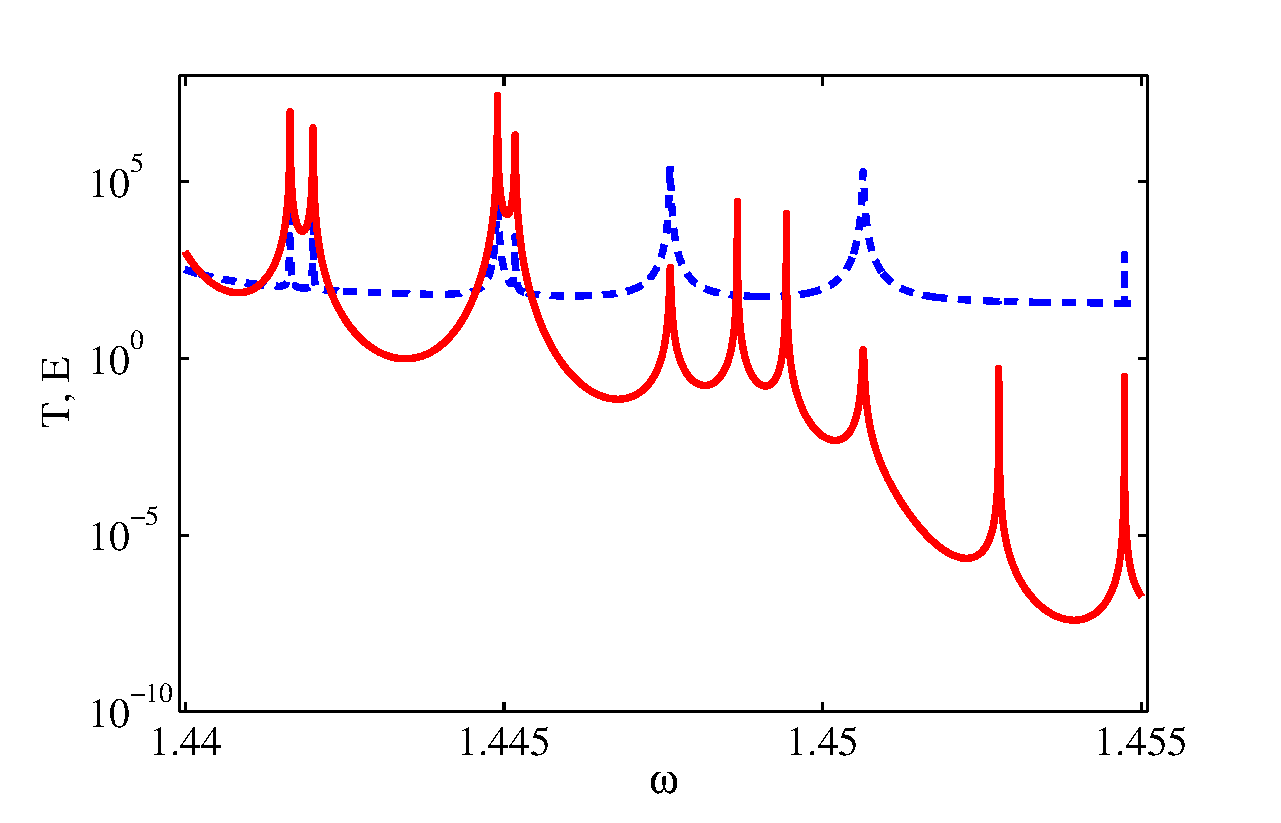
\includegraphics{pictures/tenk_energy_transmission_v_freq}}
%\begin{flushleft}(b)\end{flushleft}
%\vskip -0.1in
%\scalebox{0.38}{\includegraphics{pictures/electric_field_in_sample}}
\caption[(a) The spatially-resolved electric field in a disordered sample plotted for a range of frequencies.]{
(a) The spatially-resolved electric field in a disordered sample plotted for a range of frequencies. Five clear resonant tunneling states can be identified. 
(b) Transmission (solid line, right $y$-axis) as a function of frequency, $\tilde{T}(\omega)$, is compared to the total energy (dashed line, left $y$-axis) in the sample $\tilde{\cal E}(\omega)$ for one random realization of disorder. No one-to-one correspondence between resonant peak structures is observed.
\label{fig:electricFieldInSample}
}
\end{figure}
%%%%%%%%%%%%%%%%%%%%%%%%%%%%%%%%%%%%%%%

%%%%%%%%%%%%%%%%%%%%%%%%%%%%%%%%%%%%%%%%%%%%%%%%%%%%%%%%%
\subsection{Correlations Between \texorpdfstring{$\tilde{T}$}{T} and \texorpdfstring{$\tilde{\cal E}$}{E}}
\label{sec:correlation_te}
%%%%%%%%%%%%%%%%%%%%%%%%%%%%%%%%%%%%%%%%%%%%%%%%%%%%%%%%%

Motivated by our analysis in Section~\ref{sec:diffusion_general}, we would like to study the dependence of the ratio between transmission and stored energy in the above wave-model. Fig.~(\ref{fig:electricFieldInSample}b) shows $\tilde{T}$ and $\tilde{\cal E}$ as a function of frequency in a single disordered realization. We notice that these two parameters are not closely correlated in the localized regime. Indeed, one can see that unlike the transmission peaks, the peaks in energy are highly dissimilar with some being almost indiscernible. This disparity is an additional source of fluctuation in the ratio  $\tilde{T}/\tilde{\cal E}$. The goal of this section is to understand this behavior.

The field distribution inside the sample gives a clue why the energy may differ from resonance to resonance. At the off-resonant frequencies one observes nearly exponential decay. Whereas at or in the vicinity of a tunneling resonance, two qualitatively distinct behaviors are observed. They are illustrated in Fig.~\ref{fig:Efield_random}.

In the first scenario, c.f.~bold line in Fig.~\ref{fig:Efield_random}, the electric field grows exponentially from the incident boundary towards the localization center $x_0$ and falls off after it. For both segments the characteristic length in the exponential dependencies is set by the localization length. Such behavior is attributed\cite{1983_Azbel_zeroTemp} to the phenomenon of resonant tunneling via a localized state centered at $x_0$. 

In the other case, c.f.~thin line in Fig.~\ref{fig:Efield_random}, an additional negative exponential segment can be identified (notice the change in the direction of incidence, see figure caption). Because this type of behavior leads to significantly less energy stored inside the system, the resonances of this type do not show a pronounced spectral peak in $\tilde{\cal E}$. Although the localized states with spatial profiles as the one shown in bold in Fig.~\ref{fig:Efield_random} were studied in Ref. \cite{1983_Azbel_zeroTemp}, the second scenario exemplified by the thin line in Fig.~\ref{fig:Efield_random} was not described in that or subsequent studies by Azbel and coworkers.

We note that multi-peaked spatial intensity distribution is expected in case of so-called necklace states\cite{1987_Pendry,2005_Wiersma,2006_Genack_1d} when two or more resonant states coexist at (almost) the same energy in the given disorder realization. Such realizations, however, become less probable deep into the localization regime $L\gg\xi$ and  are not directly relevant in the current context. 

We find that, on average, roughly a half of all spectral peaks in transmission do not have the corresponding peak in $\tilde{\cal E}$. As it will become evident from the following discussion, the difference in two types of behavior in Fig.~\ref{fig:Efield_random} originates from the spatial location of the localized state. Indeed, we find that at the frequencies where peaks in transmission and energy occur simultaneously, the center of localization is located close to the incident boundary of the sample. The field distribution is qualitatively similar to the one shown in bold in Fig.~\ref{fig:Efield_random}. In contrast, at the frequencies where the peak in transmission has a significantly less pronounced (or non-distinguishable) peak in energy, the center of localization is located in the second half of the sample (closer to the exit boundary). The field distribution is qualitatively similar to the one depicted with a thin line in Fig.~\ref{fig:Efield_random}.\\

%%%%%%%%%%%%%%%%%%%%%%%%%%%%%%%%%%%%%%%
\begin{figure}
\vskip -.1in
\centerline{\rotatebox{0}{\includegraphics[width=5in]{chapters/Relation_between_transmission_and_energy_stored_in_random_media_with_gain__Phys_Rev_B/pictures/fig3_rlz2_elecfield_14_34}}}
%\scalebox{0.36}{\includegraphics{pictures/rlz2_elecfield_14_34.eps}}
\caption[Two types of the on-resonance electric field distribution inside a passive random medium with the center of localization $x_0$ in the first half (bold lines) and the second half (thin lines) of the sample ($x_0/L \approx 0.25$).]{
Two types of the on-resonance electric field distribution inside a passive random medium with the center of localization $x_0$ in the first half (bold lines) and the second half (thin lines) of the sample ($x_0/L \approx 0.25$). The second case is realized by shining the light onto the same system from the right, which is equivalent to switching boundary conditions from Eq.~(\ref{eq:basis_functions_bc_l}) to Eq.~(\ref{eq:basis_functions_bc_r}). Due to reciprocity, the value of transmission coefficient for both cases is exactly the same. However, the amount of energy stored inside the system is exponentially smaller in the second case. The latter resonance does not show noticeable peak in $\tilde{\cal E}(\omega)$. The dashed lines are the schematic envelope functions formed from segments with $\exp(\pm x/ \xi)$ spatial dependences. The parameters of the system are given in Sec.~\ref{sec:numerical_model}. 
\label{fig:Efield_random}}
\end{figure}
%%%%%%%%%%%%%%%%%%%%%%%%%%%%%%%%%%%%%%%

Realizing that our system is invariant under the time reversal transformation, one is led to the following observation. A sample with a localized state $0<x_0<L/2$ automatically yields the $L/2<x_0<L$ state in the mirror-image sample or, equivalently, by illuminating the same system from the other end as in Fig.~\ref{fig:Efield_random}. The reciprocity of the system makes the transmission coefficient the same in both cases. However, the spatial field distribution inside the system and, thus, energy stored, is dramatically different. In Appx.~\ref{app:qm_model} we show that the effect can be traced to a simple deterministic quantum model and is not specific to random systems. Indeed, the behavior observed in the models described in this section and in Appx.~\ref{app:qm_model} (c.f.~Figs.~\ref{fig:Efield_random},\ref{fig:barrierdefectlog}) can be also obtained in  other models. We checked a periodic stack of dielectric slabs as in Sec.~\ref{sec:numerical_model}, but with no disorder. Electric field distribution for the defect state created by changing the width of a single slab in the stack, appear equivalent to that in Fig.~\ref{fig:barrierdefectlog}.
 
We conclude this section with a summary of our findings: (i) Based on the analytical models we determine that the position of the center of localization ($x_0$) directly affects how much energy is stored in the system. (ii) This variation of stored energy based on the position of the center of localization explains why peaks in energy do not always correspond to the peaks in transmission. (iii) The presence of a peak in energy can be taken as an indication that the center of localization is located close to incident side of the sample. And otherwise, a peak in transmission without its counterpart in energy is indicative t the center of localization lies closer to the exit boundary.

%%%%%%%%%%%%%%%%%%%%%%%%%%%%%%%%%%%%%%%%%%%%%%%%%%%%%%%%%
\subsection{Behavior of \texorpdfstring{$\tilde{T}/\tilde{\cal E}$}{T/E} in Passive Random Medium: Spectral Vicinity of a Resonance}
\label{sec:spectral_te}

%%%%%%%%%%%%%%%%%%%%%%%%%%%%%%%%%%%%%%%%%%%%%%%%%%%%%%%%%

%%%%%%%%%%%%%%%%%%%%%%%%%%%%%%%%%%%%%%%
\begin{figure*}
\vskip -0.0in
\centerline{\rotatebox{0}{\includegraphics[width=6.75in]{chapters/Relation_between_transmission_and_energy_stored_in_random_media_with_gain__Phys_Rev_B/pictures/fig4_peaks_match_peaks_dont_match}}}
%\centerline{\scalebox{0.65}{\includegraphics{pictures/peaks_match_peaks_dont_match1}}}
\vskip 0.0in
\caption[The dependencies of $\tilde{T}(\omega )$ (a,b); envelope of the electric field  $E(x)$ (c,d); and energy in the system $\tilde{\cal E}(\omega )$ (e,f), are plotted in the spectral vicinity of a transmission resonance associated with a defect in the periodic stack of alternating dielectric layers.]{The dependencies of $\tilde{T}(\omega )$ (a,b); envelope of the electric field  $E(x)$ (c,d); and energy in the system $\tilde{\cal E}(\omega )$ (e,f), are plotted in the spectral vicinity of a transmission resonance associated with a defect in the periodic stack of alternating dielectric layers. The plots (a,c,e) and (b,d,f) are obtained for the defect located at $x_0=L/4$ and $x_0=3L/4$ respectively. In the latter case was realized by changing the direction of illumination to that given by Eq.~(\ref{eq:basis_functions_bc_r}) -- wave incident from the right -- for easy comparison with Figs.~\ref{fig:Efield_random},\ref{fig:barrierdefectlog}. In the first case, the defect center is closer to the incident boundary whereas in the second case it is closer to the exit boundary. Three sets of $E(x)$ in (c,d) are computed at the frequencies marked with dots in (a,b,e,f). The envelopes illustrate the on- and off-resonance field profiles and confirm the applicability of our approximation in Eqs.~(\ref{eq:left},\ref{eq:right},\ref{eq:startingequations},\ref{eq:energy_stored}). For the second case when the defect center is located near the exit boundary, the amount of energy stored inside the medium is dramatically lower. In this case, unlike $\tilde{T}(\omega )$, $\tilde{\cal E}(\omega )$ does not exhibit any noticeable features around $\omega_0$, compare (e) and (f). This effect leads to the asymmetry between $0<x_0<L/2$ and $L/2<x_0<L$ in the $\tilde{T}/\tilde{\cal E}$ as discussed in Sec.~\ref{sec:correlation_te} and Appx.~\ref{app:qm_model}.
\label{fig:peaksmatchnotmatch}}
\end{figure*}
%%%%%%%%%%%%%%%%%%%%%%%%%%%%%%%%%%%%%%%

In this section we employ the knowledge of the spatial profiles of the resonant states gained in Sec.~\ref{sec:correlation_te} and Appx.~\ref{app:qm_model} to obtain a closed analytical expression which qualitatively describes the behavior of $\tilde{T}/\tilde{\cal E}$ in the vicinity of a transmission resonance in terms of relevant system parameters.

In the localization regime, transmission of electromagnetic waves through a random medium occurs via tunneling or, when there exists appreciable spectral overlap with a resonant state inside the sample, via resonant tunneling. Thus, the starting point in our consideration is the simplified expression for frequency-dependent transmission coefficient in the spectral vicinity of a resonance:
\begin{equation}
\tilde{T}(\omega) = \frac{t_0^2}{\left[2(k-k_0)\Delta\right]^2+t_0^2\cosh^2\displaystyle\frac{\left|L-2x_0\right|}{\xi} }
\label{eq:transmission}
\end{equation}
where $k=\omega/c$ and $t_0=\exp(-L/\xi)$ determines the value of the transmission away from the resonance at $k_0$. $\Delta$ is a quantity with the dimensionality of length. It has the physical meaning of the characteristic spatial extent of the region which serves as the resonant ``cavity"\cite{2008_Bliokh}. $\Delta$ is a model dependent quantity which is related to the cavity width in deterministic models, see e.g. \cite{1994_Pendry,2001_Deych_mqw}. In the case of random media, $\Delta$ is the length of the locally transparent region in the sample which serves as a cavity created due to random fluctuation of the disorder. In this system $\Delta$ is comparable to the localization length\cite{2004_Bliokh_wavelet}.

Of course, even within framework of the simplistic model of Appx.~\ref{app:qm_model} the true expression for the transmission coefficient is more complex than Eq.~(\ref{eq:transmission}). However, the latter adequately captures the functional dependence on such parameters as $k-k_0,x_0,\xi$ and ,$L$: Eq.~(\ref{eq:transmission}) follows from the exact solution in the limit $\left|k-k_0\right|\leq\delta k$ and $L\gg\xi$ (which also leads to $\delta k\ll k_0$ condition). Here $\delta k$ is the spectral width of the resonance.

Qualitative analogy between a disordered 1D random medium and a deterministic quantum model similar to that in Appx.~\ref{app:qm_model} was demonstrated in Ref. \cite{2004_Bliokh_wavelet}. Therefore, we expect Eq.~(\ref{eq:transmission}) to be also qualitatively applicable in the random layered medium of Sec.~\ref{sec:numerical_model}.

We note two important properties of Eq.~(\ref{eq:transmission}). First, the maximum (resonant) value of the transmission at $\omega =\omega_0$ is determined by the location of the cavity as $\tilde{T}(\omega_0)=\cosh^{-2}\left(\left|L-2x_0\right|/\xi\right)$. It turns to unity when $x_0=L/2$. Secondly, when the frequency of the incident light is detuned from the resonance $\left|\omega-\omega_0\right|\gg\delta\omega$, the above expression loses it validity -- the presence of the other resonant states must be accounted for.

%%%%%%%%%%%%%%%%%%%%%%%%%%%%%%%%%%%%%%%
\begin{figure}
\centerline{\rotatebox{0}{\includegraphics[width=3.5in]{chapters/Relation_between_transmission_and_energy_stored_in_random_media_with_gain__Phys_Rev_B/pictures/fig5_energy_distribution_and_TE_dual_axis}}}
%\vskip -0.0cm
%\centerline{
%\scalebox{0.5}{\includegraphics{pictures/energy_distribution_and_TE_dual_axis.eps}}}
%\vskip -0.0cm
\caption[The solid line plots $\tilde{\cal E}(\omega_0,x_0)$ from Eq.~(\ref{eq:energy_stored}).]{The solid line plots $\tilde{\cal E}(\omega_0,x_0)$ from Eq.~(\ref{eq:energy_stored}). The energy stored inside a random medium falls off sharply (exponentially) when the center of localization $x_0$ increases beyond $L/2$ and reaches the off-resonant value for $x_0>2L/3$. The dashed line with the right $y$-axis represents the ratio between $\tilde{T}(\omega_0,x_0)$ in Eq.~(\ref{eq:transmission}) and  $\tilde{\cal E}(\omega_0,x_0)$ in Eq.~(\ref{eq:energy_stored}). The ratio peaks at the same value of $x_0/L=2/3$. The latter value does not depend on either the localization length $\xi$ or the system length $L$. \label{fig:energydistrib}}
\end{figure}
%%%%%%%%%%%%%%%%%%%%%%%%%%%%%%%%%%%%%%%

%\begin{widetext}
From analysis of random and deterministic models in Sec.~\ref{sec:correlation_te} and Appx.~\ref{app:qm_model}, c.f.~Figs.~\ref{fig:Efield_random},\ref{fig:barrierdefectlog}, we approximate the envelope of the {\it on-resonance} electric field distribution as
\begin{equation}
E(x,\omega_0) = \left\{
\begin{array}{l l}
B(\omega_0,x_0) \exp [ (x-x_0)/\xi ] &\quad 0 < x < x_0 \\
C(\omega_0,x_0) \exp [-(x-x_0)/\xi ] &\quad x_0 < x < L\\
\end{array} \right.
\label{eq:left}
\end{equation}
for $x_0<L/2$; and
\begin{equation}
E(x,\omega_0) = \left\{
\begin{array}{l l}
 A(\omega_0,x_0) \exp [-x      /\xi ] &\quad 0 < x < x_T(\omega_0)   \\
 B(\omega_0,x_0) \exp [ (x-x_0)/\xi ] &\quad x_T(\omega_0) < x < x_0 \\
 C(\omega_0,x_0) \exp [-(x-x_0)/\xi ] &\quad x_0 < x < L \\
\end{array} \right.
\label{eq:right}
\end{equation}
for $x_0>L/2$. Here $A,B,C$ are constants to be determined from the continuity conditions. At the boundaries we set $E(x=0)=1$ and $E(x=L)=\tilde{T}^{1/2}(\omega_0)$. Noticing that $E(x=L,\omega_0)\approx\exp\left[ -|2x_0-L|/\xi\right]$ yields the following expression for the location for the turning point, $x_T(\omega_0)=2x_0-L$, in the case of Eq.~(\ref{eq:right}). In the context of light propagation in random media, such as in Sec.~\ref{sec:numerical_model}, the Eqs.~(\ref{eq:left},\ref{eq:right}) have the meaning of the typical envelope of the true spatial distribution of the electric field in the random systems with the same values of the parameters $(\omega-\omega_0),x_0,\xi$, and $L$.

In both cases above, away from the resonant frequency $k_0$, we see three distinct regions:
\begin{equation}
E(x) = \left\{
\begin{array}{l l}
A(\omega,x_0) \exp[- x     /\xi]  &\quad 0 < x < x_T(\omega)    \\
B(\omega,x_0) \exp[ (x-x_0)/\xi]  &\quad x_T(\omega) < x < x_0  \\
C(\omega,x_0) \exp[-(x-x_0)/\xi]  &\quad x_0 < x < L    \\
\end{array} \right. 
\label{eq:startingequations}
\end{equation}
where $x_T(\omega)$ again has to be determined from the boundary conditions $E(x=0)=1$ and $E(x=L)=T^{1/2}(\omega)$. Fig.~\ref{fig:peaksmatchnotmatch} illustrates the obtained electric field distribution for both $x_0<L/2$ and $x_0>L/2$ cases. It also makes it clear that the energy stored inside the sample varies from resonance to resonance due to the position of the center of localization $x_0$. Indeed, integrating Eqs.~(\ref{eq:left},\ref{eq:right}) gives us the sought expression for $\tilde{\cal E}(\omega)$. At $\omega=\omega_0$ it simplifies to
\begin{equation}
\tilde{\cal E}(x_0)\propto\left\{
\begin{array}{l l}
2\tilde{T}(\omega)\exp\left[2(L-x_0)/\xi\right]-1- \tilde{T}(\omega) & \quad 0  < x_0 < L/2 \\
2\tilde{T}(\omega)\exp\left[2(L-x_0)/\xi\right]+1-3\tilde{T}(\omega) & \quad L/2< x_0 < L   \\
\end{array}
\right.
\label{eq:energy_stored}
\end{equation}
%\end{widetext}
This expression is plotted in Fig.~\ref{fig:energydistrib}. It shows dramatic disparity between the cases $x_0<L/2$ and $x_0>L/2$. Eq.~(\ref{eq:energy_stored}) also shows that even at the frequency of the resonance the amount of energy stored inside the system becomes essentially the same as an off-resonant case for $x_0>2L/3$. The latter value of $x_0$ is independent of any other parameters of the systems such as $\xi$, $L$, etc.

When expressions in Eqs.~(\ref{eq:transmission},\ref{eq:energy_stored}) are combined to form the ratio $\tilde{T}/\tilde{\cal E}$, one obtains highly asymmetric dependence on the position of the center of localization $x_0$, c.f.~Fig.~\ref{fig:energydistrib}. The ratio increases approximately exponentially for $0<x_0<2L/3$ and falls off also exponentially in the interval $2L/3<x_0<L$. This observation confirms our previous conclusion on the sensitivity of the $\tilde{T}/\tilde{\cal E}$ on $x_0$. In the next section we study the effect of (linear) optical amplification on this quantity.

%%%%%%%%%%%%%%%%%%%%%%%%%%%%%%%%%%%%%%%%%%%%%%%%%%%%%%%%%
\subsection{Behavior of \texorpdfstring{$\tilde{T}/\tilde{\cal E}$}{T/E} in Active Random Medium} 
\label{sec:localization_gain}
%%%%%%%%%%%%%%%%%%%%%%%%%%%%%%%%%%%%%%%%%%%%%%%%%%%%%%%%%

%%%%%%%%%%%%%%%%%%%%%%%%%%%%%%%%%%%%%%%%%%%%%%%%%%%%%%%%%%%%%%
\begin{figure}
\centerline{\rotatebox{0}{\includegraphics[width=3.25in]{chapters/Relation_between_transmission_and_energy_stored_in_random_media_with_gain__Phys_Rev_B/pictures/fig6a_periodic_34_defect_passive_to_gain2}}}
\centerline{\rotatebox{0}{\includegraphics[width=3.25in]{chapters/Relation_between_transmission_and_energy_stored_in_random_media_with_gain__Phys_Rev_B/pictures/fig6b_periodic_14_defect_passive_to_gain2}}}
%\begin{flushleft}
%(a)
%\end{flushleft}
%\vskip -0.7cm
%\centerline{\scalebox{0.35}{\includegraphics{pictures/periodic_34_defect_passive_to_gain2.eps}}}
%\begin{flushleft}
%(b)
%\end{flushleft}
%\vskip -0.7cm
%\centerline{\scalebox{0.35}{\includegraphics{pictures/periodic_14_defect_passive_to_gain2.eps}}}
%\vskip -0.0cm
\caption[An illustration of the effect gain on the electric field distribution in a 1D random medium.]{An illustration of the effect gain on the electric field distribution in a 1D random medium. A periodic stack of alternating dielectric layers with a defect at $x_0=L/4$ is considered. As discussed in Sec.~\ref{sec:correlation_te}, such a model qualitatively describes the field profiles (such as those in Fig.~\ref{fig:Efield_random}) in random media. Panels (a) and (b) show the field envelopes obtained when the system is illuminated (at resonant frequency) from the left and right respectively. Dashed lines correspond to the passive medium. The solid curves (from bottom up) are obtained for $l_{g,cr}/l_g$ equal to $0.5,\ 0.9,\ 0.99$ in (a) and $0.85,\ 0.95,\ 0.98,\ 0.99$ in (b). The field distribution in (b) shows a dramatic modification with an increase of gain.\label{fig:localization_gain}}
\end{figure}
%%%%%%%%%%%%%%%%%%%%%%%%%%%%%%%%%%%%%%%%%%%%%%%%%%%%%%%%%%%%%%

As we observed in Sec.~\ref{sec:diffusion_general}, a change in $T/{\cal E}$ with gain is indicative of a modification of the intensity profile inside a diffusive slab. Similar conclusions can be made in the localized regime. Our simulations demonstrate that a change in $\tilde{T}/\tilde{\cal E}$ indeed signifies the modification of the field distribution inside the random medium. Interestingly, we find that such modifications can be very dramatic in the localization regime. 

To illustrate the effect of linear gain on the spatial profile of the EM field, we employ the deterministic (non-random) model of the periodic stack of alternating dielectric layers with a defect (see Sec.~\ref{sec:spectral_te}). The gain is simulated by adding a spatially constant imaginary part to the dielectric constant of the medium  as $\epsilon(x)\rightarrow\epsilon(x)+i\alpha$. As previously discussed in Sec.~\ref{sec:intro}, such modeling of stimulated amplification is justified for values of gain up to the threshold for random lasing.

The results of our simulations are plotted on Fig.~\ref{fig:localization_gain}. One can see the strong enhancement of the electric field in the vicinity of the center of localization for the defect located in the farther half of the sample. Such enhancement is accompanied by the shift of the turnaround point $x_T$, where the negative exponential crosses over to the positive exponential behavior, towards the sample boundary. At a certain value of the gain parameter, the negative exponential segment of the $E(x)$ disappears and the field profile assumes the limiting shape which coincides with that under excitation from the opposite boundary of the system. The above observations also hold in the random medium model of Sec.~\ref{sec:correlation_te}. 

At first glance, the modification of the field profile due to gain seems to disagree with the conclusions in Refs.~\cite{2002_Jiang_Loc_Modes_Lasing,2002_Sebbah_Vanneste,2005_Vanneste} where (in localized regime) little or no change in the field pattern was found with an increase of amplification. The apparent discrepancy can be explained if one compares the methods used to excite the system. In our work, we consider the transmission experiment setup, whereas in the previous works \cite{2002_Jiang_Loc_Modes_Lasing,2002_Sebbah_Vanneste,2005_Vanneste} the system is excited throughout its entire volume or relatively close to the center of localization. Under such excitation conditions, the situation shown in Fig.~\ref{fig:localization_gain}a is always realized \cite{2010_Payne_loc_criterion}. We also note that the mode distribution in Fig.~\ref{fig:localization_gain}b is observed to converge to that in Fig.~\ref{fig:localization_gain}a when the gain approaches its critical value. Then the field distribution is maintained by the gain with little reliance on the incident energy.

%%%%%%%%%%%%%%%%%%%%%%%%%%%%%%%%%%%%%%%%%%%%%%%%%%%%%%%%%
%\subsection{Gain-induced electric field modifications\label{sec:localization_gain_explained}} 
%%%%%%%%%%%%%%%%%%%%%%%%%%%%%%%%%%%%%%%%%%%%%%%%%%%%%%%%%

%%%%%%%%%%%%%%%%%%%%%%%%%%%%%%%%%%%%%%%%%%%%%%%%%%%%%%%%%%%%%%
\begin{figure*}
%\vskip -0.0cm
\centerline{\rotatebox{0}{
\includegraphics[width=2in]{chapters/Relation_between_transmission_and_energy_stored_in_random_media_with_gain__Phys_Rev_B/pictures/fig7a_alpha_beta_electric_field}
\includegraphics[width=2in]{chapters/Relation_between_transmission_and_energy_stored_in_random_media_with_gain__Phys_Rev_B/pictures/fig7b_alpha2_beta2}
\includegraphics[width=2in]{chapters/Relation_between_transmission_and_energy_stored_in_random_media_with_gain__Phys_Rev_B/pictures/fig7c_alpha1_beta1}
}}
%\centerline{
%\scalebox{0.33}{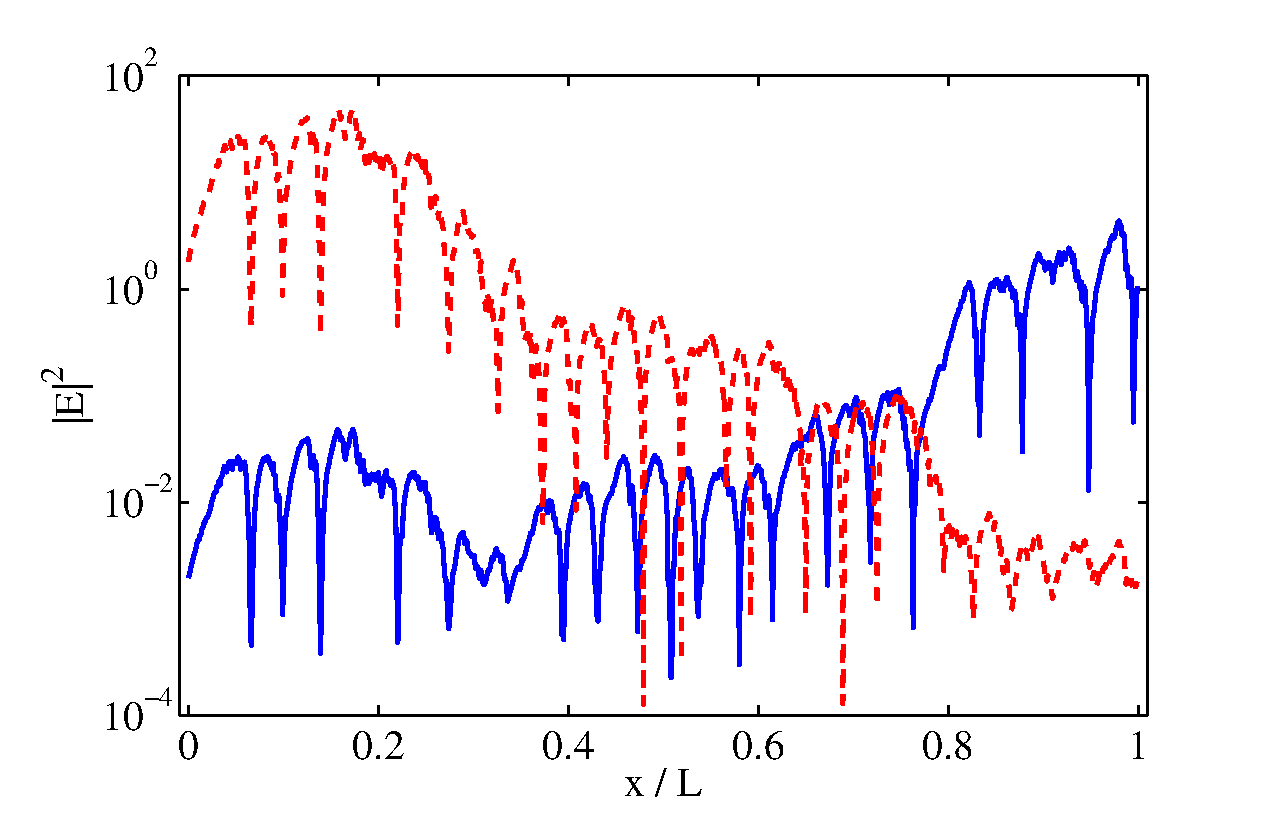
\includegraphics{pictures/alpha_beta_electric_field}}
%\scalebox{0.33}{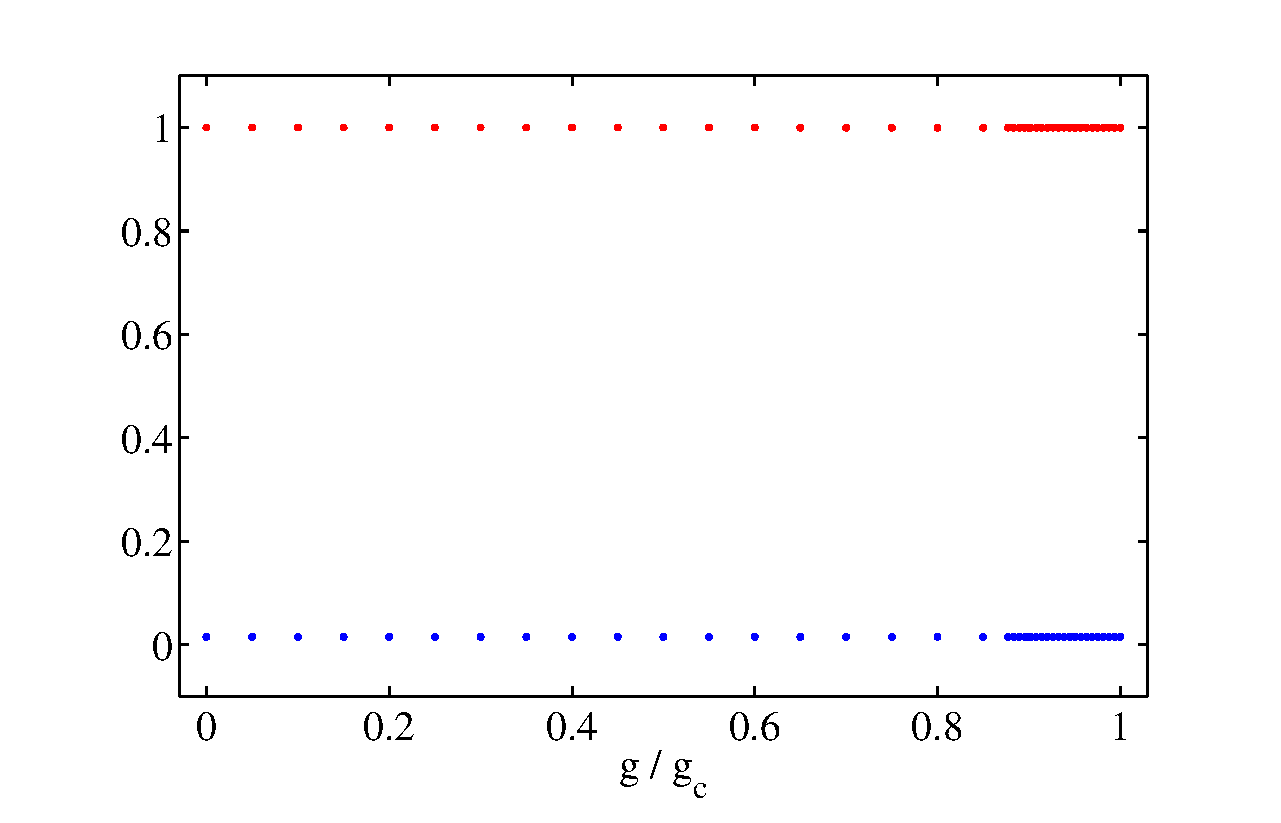
\includegraphics{pictures/alpha2_beta2}}
%\scalebox{0.33}{\includegraphics{pictures/alpha1_beta1}}}
%\vskip -0.0cm
\caption[Panel (a) plots $E_{L,R}(x,\omega_c)\equiv  E^{(L,R)}(x,\omega_c,\alpha=0)$ defined by the boundary conditions in Eqs.~(\ref{eq:basis_functions_bc_l},\ref{eq:basis_functions_bc_r}), see text for notations.]{Panel (a) plots $E_{L,R}(x,\omega_c)\equiv  E^{(L,R)}(x,\omega_c,\alpha=0)$ defined by the boundary conditions in Eqs.~(\ref{eq:basis_functions_bc_l},\ref{eq:basis_functions_bc_r}), see text for notations. For non-zero gain, $\alpha>0$, the electric field distributions $E^{(L,R)}(x,\omega_c,\alpha)$ are found to be qualitatively similar to those in Fig.~\ref{fig:localization_gain}. We decompose them in terms of the functions shown in (a), and the resulting coefficients $C_{L,R}^{(L)}(\alpha)$ and $C_{L,R}^{(R)}(\alpha)$, defined in Eq.~(\ref{eq:C_completeness}), are plotted in (b) and (c) respectively. We find that the close resemblance between $E_{L}(x,\omega_c)$ and $E^{(c)}(x,\omega_c)$ (the solution in the closed system) makes it the dominant limiting profile in the vicinity of threshold for random lasing, regardless of the direction of excitation. In all three panels, thick / thin curve and large / small symbols refer to  $E_{L}(x,\omega_c)$ / $E_{R}(x,\omega_c)$.\label{fig:alphabeta}}
\end{figure*}
%%%%%%%%%%%%%%%%%%%%%%%%%%%%%%%%%%%%%%%%%%%%%%%%%%%%%%%%%%%%%%

Below we provide a simple physical picture for the modification of the electric field with an increase of optical gain. 

We start by considering the passive system. We recall that our sample is an open system where a wave is incident onto the system and one observes the scattered (reflected and transmitted) signals.  Under these conditions a continuous wave (CW) solution of the Maxwell equations with the given frequency is a complex function. The complex conjugate of such a solution is also a (linearly independent) solution for the same frequency. In general, any two (because Maxwell's equation is the second order differential equation) linearly independent solutions can be used as a basis for expressing any other solution at the same frequency $\omega$. 

Now we would like to consider two particularly important solutions of the Maxwell equation in the random 1D sample with the boundary conditions defined by Eqs.~(\ref{eq:basis_functions_bc_l},\ref{eq:basis_functions_bc_r}). They correspond to the left- and right-incident cases respectively as considered in Sec.~\ref{sec:correlation_te} and Appx.~\ref{app:qm_model} with $r_{L,R}(\omega),t_{L,R}(\omega)$ being the corresponding amplitude reflection and transmission coefficients. To check the linear independence of these two solutions it suffices to verify that their Wronskian (it is independent of $x$ in our model of disorder $\epsilon(x)$) is non-zero for one particular value of $x$. At $x=0$ the Wronskian can be computed from the boundary conditions  Eqs.~(\ref{eq:basis_functions_bc_l},\ref{eq:basis_functions_bc_r}) as $-2it_R(\omega)\omega/c\neq 0$.

At some special frequencies $\omega_c$, a linear combination  $E^{(c)}(x,\omega_c)=C_L^{(c)} E_{L}(x,\omega_c)+C_R^{(c)} E_{R}(x,\omega_c)$ can be formed such that conditions $E^{(c)}(x=0,\omega_c)=0$ and $E^{(c)}(x=L,\omega_c)=0$ are satisfied simultaneously. Such $\omega_c$'s  correspond to the true eigen-modes of the closed system -- the system defined by $\epsilon(0\leq x\leq L)$ with zero (reflecting) boundary conditions at $x=0,L$. We numerically obtained such solutions in our 1D random model and found that the single cusp solution (similar to $E_{L}(x,\omega_c)$ depicted with thick lines in Figs. (\ref{fig:Efield_random},\ref{fig:barrierdefectlog})) makes the dominant contribution to $E^{(c)}(x,\omega_c)$. This may explain why the other profile with the negative exponential tunneling segment (similar to $E_{R}(x,\omega_c)$ depicted with thin lines in Figs. (\ref{fig:Efield_random},\ref{fig:barrierdefectlog})) is not seen under uniform excitation as in Refs.~\cite{2002_Jiang_Loc_Modes_Lasing,2002_Sebbah_Vanneste,2005_Vanneste}.

We now turn to the case of random medium with gain, $\alpha>0$, and consider the spatial field distribution obtained when system is illuminated from the left, $E^{(L)}(x,\omega_c,\alpha)$, and from the right $E^{(R)}(x,\omega_c,\alpha)$, c.f.~Fig.~\ref{fig:localization_gain}. In this case, the distributions can no longer, strictly speaking, be expressed in terms of $E_{L,R}(x,\omega_c)\equiv  E^{(L,R)}(x,\omega_c,\alpha=0)$. However, in the regime of localized transport considered here, $\alpha<\alpha_{cr}\ll\omega_c$, the deviation from completeness of the basis $E_{L,R}(x,\omega_c)$ are to remain small so that  the dependence of $E(x,\omega_c,\alpha)$ on gain can be still reliably approximated by $\alpha$-dependent $C_{L}(\alpha)$,$C_{R}(\alpha)$:
\begin{equation}
E(x,\omega_c,\alpha)\simeq C_L(\alpha) E_{L}(x,\omega_c)+C_R(\alpha) E_{R}(x,\omega_c).
\label{eq:C_decomposition}
\end{equation}
The applicability of the approximation in Eq.~(\ref{eq:C_decomposition}) is verified numerically by computing  
\begin{equation}
C_{L,R}^{(L,R)}(\alpha)=\int_{0}^{L} E^{(L,R)}(x,\omega_c,\alpha)E_{L,R}^*(x,\omega_c)dx.
\label{eq:C_completeness}
\end{equation}
Figs.~\ref{fig:alphabeta}b,c show $C_{L,R}^{(L)}(\alpha)$ and $C_{L,R}^{(R)}(\alpha)$ respectively. Here we select a random realization with a localization center at $x_0\sim L/4$ where passive profiles, depicted in Fig.~\ref{fig:alphabeta}a, show the two characteristic shapes considered in Figs.~\ref{fig:Efield_random},\ref{fig:barrierdefectlog},\ref{fig:localization_gain}. When gain is added to the system, we observe that $E^{(L)}(x,\omega_c,\alpha)\propto E_{L}(x,\omega_c)$ for all values of gain, c.f.~Fig.~\ref{fig:alphabeta}b. In contrast, $E^{(R)}(x,\omega_c,\alpha)$ exhibited a crossover behavior from $E^{(R)}(x,\omega_c,\alpha)\propto E_{R}(x,\omega_c)$ for small $\alpha$, to $E^{(R)}(x,\omega_c,\alpha)\propto E_{L}(x,\omega_c)$ in the vicinity of lasing threshold. This result corroborates the findings of the previous Sec.~\ref{sec:localization_gain}, c.f.~Fig.~\ref{fig:localization_gain}, that the modification of the electric field distribution with an increase of amplification strength is possible in the localized regime. Here we have shown that it occurs due to the existence of two possible mode profiles (at the same frequency), of which only one strongly resembles the solution of the system with closed-boundaries. It is the function with no turning point which defines the lasing mode in the vicinity the threshold for random lasing. 

Finally, we note that the solutions $E_{L,R}(x,\omega)$ should not be confused with the quasi-mode $E(x,\omega_c+i\varepsilon)$ of the system with the outgoing boundary conditions obtained at the complex frequency $\omega_c+i\varepsilon$ where e.g. transmission becomes singular. Such quasi-modes are often invoked in discussion of modes involved in random lasing. However, for a uniform gain in the form $\epsilon(x)(1+i\alpha)$ the dominant mode profile $E^{(L)}(x,\omega_c,\alpha_{cr})$ does indeed coincide with the quasi-mode due to equivalence between $\epsilon(x)(1+i\alpha)\omega_c/c$ and $\epsilon(x)(\omega_c+i\varepsilon)/c$.

%%%%%%%%%%%%%%%%%%%%%%%%%%%%%%%%%%%%%%%%%%%%%%%%%%%%%%%%%
\section{DISCUSSION AND OUTLOOK}
\label{sec:discussion_TE}
%%%%%%%%%%%%%%%%%%%%%%%%%%%%%%%%%%%%%%%%%%%%%%%%%%%%%%%%%

In this work we have studied the relationship between transmission of light through passive and active random media and the amount of the electromagnetic energy stored in it. The ratio of these two quantities does not show a tendency to diverge with an increase of the gain strength and, thus, is a good candidate for a parameter which can quantify the enhancement of the mesoscopic phenomena  random medium with amplification \cite{2004_Yamilov_intensity,2005_Yamilov_correlations,2006_Yamilov_conductance}. 

In Sec.~\ref{sec:diffusion_section} we established a connection between the ratio of the ensemble-averaged quantities $T/{\cal E}$ and the spatially dependent diffusion coefficient, Eq.~(\ref{eq:TE_vs_D}), in a passive random medium. This relation implies that a deviation (decrease) of $T/{\cal E}$ from the value given by that expression with the classical un-renormalized diffusion coefficient $D(z)\equiv D_0=c\ell/3$ may be attributed to the localization effects. 

In Sec.~\ref{sec:diffusion_general} we obtained the expressions for $T$ and ${\cal E}$ in the diffusive random medium with amplification. Drawing an analogy with the passive systems, we conjecture that the decrease in $T/{\cal E}$ below the level established by Eq.~(\ref{eq:TE_analytical}) may be interpreted as a manifestation of an enhancement of mesoscopic correction in transport in systems with gain. We plan to examine the validity of this conjecture in future work.

We argue that in random media with strong sample-to-sample fluctuations, such as systems with large gain or strongly scattering media, the ratio between $\tilde{T}$ and $\tilde{\cal E}$ from the same disorder realization needs to be formed before performing statistical averages. This led us to investigate the relationship between these two parameters in systems in the localized regime, c.f.~Sec.~\ref{sec:localization_passive}. Although the ratio $\tilde{T}/\tilde{\cal E}$ does not tend to diverge when gain is added, it exhibits additional fluctuations due to the sample orientation (or, equivalently, the direction of the incident wave) even in the passive system, c.f.~Sec.~\ref{sec:correlation_te}. In Sec.~\ref{sec:spectral_te},\ref{app:qm_model} we attribute the fluctuations to the dependence on the position of the localization center inside the system. This is unlike the transmission $\tilde{T}$, which is independent of direction of illumination (because of reciprocity) -- it is the same for both field distributions depicted in Fig.~\ref{fig:Efield_random}. One possibility to generalize the transmission in the active random media, while retaining the desired cancellation  of the divergence in the vicinity of the threshold for random lasing, is to consider the modified parameter similar to the one studied in this work: $\tilde{T}_G(\alpha)=\left(\tilde{T}(\alpha)/\tilde{\cal E}(\alpha)\right)\times\tilde{\cal E}_0$. Here $\tilde{\cal E}_0\equiv\tilde{\cal E}(\alpha=0)$ is the energy stored in the random medium with no gain. All quantities entering the expression for $\tilde{T}_G$ should be evaluated for each disorder realization prior to any statistical analysis. By construction, $\tilde{T}_G(\alpha)$ reduces to the transmission in a 1D system without gain ($\alpha\rightarrow 0$) and can be generalized in the higher dimensional systems as the (average) dimensionless conductance upon statistical averaging. Hence, one can refer to $T_G$ as generalized transmission (conductance).

In future, we plan to investigate both theoretically and experimentally the statistical properties of both $\tilde{T}(\alpha)/\tilde{{\cal E}}(\alpha)$ and $T_G(\alpha)$ in random medium with gain. Experimentally, all quantities entering their definition can be determined from near-field scanning measurements in two-dimensional random media -- structurally disordered semiconductor films. This opens up a possibility to corroborate and extend the results of this study. 

%%%%%%%%%%%%%%%%%%%%%%%%%%%%%%%%%%%%%%%%%%%%%%%%%%%%%%%%%
\section{ACKNOWLEDGMENTS}
%%%%%%%%%%%%%%%%%%%%%%%%%%%%%%%%%%%%%%%%%%%%%%%%%%%%%%%%%
 
This work was supported by National Science Foundation Grant Nos. DMR-0704981 and DMR-0808937. The numerical
results obtained at the Tera-Grid, Grants No. DMR-090132 and No. DMR-100030. AY is grateful to S. Skipetrov, A. Lagendijk and B. van Tiggelen for valuable comments.

\section{APPENDIX}
%\appendix

\subsection{Derivation of Equation~(\ref{eq:TE_vs_D})}
\label{app:Dz_derivation}
We consider a slab geometry, where we explicitly  separate the coordinate $z$ normal to the slab from the perpendicular component ${\bf \rho}$ as ${\bf r}=({\bf \rho},z)$. Assuming no dependence on ${\bf \rho}$ allows us to rewrite Eq.~(\ref{eq:Jflux}) in the form
\begin{equation}
\langle J_z(z)\rangle=
\displaystyle -D(z)\frac{d\langle {\cal W}(z)\rangle}{dz}.
\label{eq:Jfluxz}
\end{equation}
Independence of ${\bf \rho}$ is insured for the plane-wave illumination boundary condition which we assume here. 

In the CW regime when the energy density ${\cal W}(z)$ is stationary, $\partial \langle {\cal W}(z)\rangle/\partial t=0$, it follows from Eq.~(\ref{eq:Jflux_conserv}) that the $z$-component of flux is constant for $z>z_p\sim\ell$. The value of the constant can be obtained from the boundary condition at $z=L$ as
\begin{equation}
\langle J_z(z)\rangle=\left\{
\begin{array}{l l}
\langle J_z(L)\rangle\equiv J_0 T,&\quad z_p<z<L\\
\langle J_z(0)\rangle\equiv -J_0 R,&\quad 0<z<z_p\\
\end{array} \right.
\label{eq:Jfluxz_const}
\end{equation}
where $T$ is the transmission coefficient. Furthermore, by integrating Eq.~(\ref{eq:Jflux_conserv}) over the entire system we obtain the flux conservation $\langle J_z(L)\rangle -\langle J_z(0)\rangle =J_0 T-(-J_0 R)=J_0(T+R)=J_0$.

After establishing Eq.~(\ref{eq:Jfluxz_const}), we can return to finding the energy stored inside the system from Eq.~(\ref{eq:Jfluxz}). An integration over $z$ gives
\begin{equation}
\displaystyle\int_z^L\frac{\langle J_z(z^\prime)\rangle dz^\prime}{D(z^\prime)}=-\langle {\cal W}(L)\rangle + \langle {\cal W}(z)\rangle.
\label{eq:E1}
\end{equation}
The energy density $\langle {\cal W}(L)\rangle$ at the right boundary can be expressed in terms of right- and left-propagating fluxes $\langle J_+(L)\rangle=J_0T$, $\langle J_-(L)\rangle=0$ using Eqs.~(\ref{eq:diffusive_flux}). We obtain $\langle {\cal W}(L)\rangle=2J_0T/c$. To take advantage of the fact that $\langle J_z(z)\rangle$ is piecewise constant, c.f.~Eq.~(\ref{eq:Jfluxz_const}), we have to neglect by $0<z<z_p$ contribution. This introduces an error $\propto z_p/L\sim\ell/L\ll 1$, but at the same time allows one to factorize $T$ and $D(z)$ contributions as
\begin{equation}
J_0T\left[\displaystyle\int_z^L\frac{dz^\prime}{D(z^\prime)}+2/c\right]= \langle {\cal W}(z)\rangle.
\label{eq:E1a}
\end{equation}
Before proceeding further, we note that the second term in the brackets is of the same order $\sim \ell/L$ as the term  omitted in arriving to the above expression. Hence, $2/c$ contribution has to be dropped as well.

A subsequent integration of Eq.~(\ref{eq:E1a}) gives 
\begin{equation}
J_0T\displaystyle\int_{0}^{L}\int_{z}^{L}\displaystyle\frac{1}{D(z^\prime)}dz^\prime dz=
\displaystyle\int_0^L \langle {\cal W}(z)\rangle dz
\equiv{\cal E}
\label{eq:E2}
\end{equation}
Taking advantage of the system symmetry, $D(z)=D(L-z)$, the double integration can be further simplified as
\begin{eqnarray}
\displaystyle\int_{0}^{L}\int_{z}^{L}\displaystyle\frac{1}{D(z^\prime)}dz^\prime dz &=&\frac{1}{2}\displaystyle\int_{0}^{L}\int_{0}^{L}\displaystyle\frac{1}{D(z^\prime)}dz^\prime dz \nonumber\\
&=&\frac{L}{2}\int_{0}^{L}\displaystyle\frac{1}{D(z)}dz.
\label{eq:E3}
\end{eqnarray}
After normalizing the integral so that it yields unity in the case when the wave interference effects are neglected, $D(z)=D_0\equiv c\ell/3$, we obtain Eq.~(\ref{eq:TE_vs_D}).

\subsection{Dependence of \texorpdfstring{$\tilde{T}/\tilde{\cal E}$}{T/E} on Position of the Defect State: Non-random Model}
\label{app:qm_model}
%%%%%%%%%%%%%%%%%%%%%%%%%%%%%%%%%%%%%%%%%%%%%%%%%%%%%%%%%

In this section we show that the origin of orientation-dependent energy content as in Fig.~\ref{fig:Efield_random} can be traced to a quantum mechanical tunneling problem in the system which is comprised of a potential well surrounded by two barriers of finite height. 

A clarification is in order. There is no one-to-one analogy between the solutions of Schr\"{o}dinger and Helmholtz equations\cite{2004_dragoman_book}. Indeed, John \cite{1991_John} pointed out that the effective energy of photons always exceeds the highest effective potential barrier so that concept of quantum mechanical tunneling cannot be, strictly speaking, applied to the electromagnetic waves. However, in the dielectrics with an inherent periodicity\cite{1987_John} (e.g. disordered photonic crystals), the negative energy and, thus, tunneling regime can be recovered. To achieve this formally, the periodicity has to be eliminated via a suitable effective-medium transformation, as in e.g. Refs \cite{1994_Sipe,2004_Bliokh_wavelet,2008_Yamilov_JoSAB}. 

Here we consider the potential which consists of two barriers separated by a well. In particular, we will be interested in comparing spatial dependence of the wavefunction for the well located in the first (at $x_0=L/4$) and the second (at $x_0=3L/4$) half of of the system. The potential profile is shown with dashed line in Fig.~\ref{fig:barrierdefectlog}. As in Sec.~\ref{sec:correlation_te}, $x_0=3L/4$ is realized by changing the direction of illumination.

The straightforward solution of the Schr\"{o}dinger equation leads to a transmission resonance (due to resonant tunneling via quantum state in the well) at the energy below the barriers height. Fig.~\ref{fig:barrierdefectlog} plots the corresponding wave functions at the energy of the resonance. As it is clearly visible in logarithmic scale, the transmission through the barrier is the same for the well at $L/4$ and $3L/4$, despite of the drastically different amplitude of the wave function in the sample. The structure of the wavefunctions is qualitatively similar to that of the periodic-on-average random medium defined in Sections \ref{sec:numerical_model},\ref{sec:correlation_te}. In the case of $x_0=3L/4$ defect, the exponential decay extends from the incident boundary through $x_T$, where $x_T$ is the turning point. The position of $x_T$ is determined by ensuring that the transmission coefficient remains the same in both cases shown in Fig.~\ref{fig:barrierdefectlog}, as required by the reciprocity of the problem.

%%%%%%%%%%%%%%%%%%%%%%%%%%%%%%%%%%%%%%%
\begin{figure}%[t]
\vskip -0.8cm
\centerline{\rotatebox{0}{\includegraphics[width=3.25in]{chapters/Relation_between_transmission_and_energy_stored_in_random_media_with_gain__Phys_Rev_B/pictures/fig8_barrier_defect_at_14_and_34_waveform_log_chopped}}}
%\vskip -0.0in
%\scalebox{0.37}{\includegraphics{pictures/barrier_defect_at_14_and_34_waveform_log_chopped.eps}}
%\vskip -0.2in
\caption[Solution of the Schr\"{o}dinger equation for a potential barrier shown with the dashed line.]{Solution of the Schr\"{o}dinger equation for a potential barrier shown with the dashed line. The wavefunction is plotted at resonant energy of the quasi-bound state associated with the well inside the potential barrier. The obtained spatial dependence in cases of the wave incident from the left (thick line) and the right (thin line) are qualitatively similar to those in Fig.~\ref{fig:Efield_random}.\label{fig:barrierdefectlog}}
\end{figure}
%%%%%%%%%%%%%%%%%%%%%%%%%%%%%%%%%%%%%%%

The non-monotonic behavior of the wavefunction can be understood intuitively as follows. In the barrier regions there exist two eigen-solutions with exponentially increasing and exponentially decreasing amplitudes (in the electromagnetic problem, the envelope of the electric field plays the role of the amplitude). Balance between these two components is determined from the boundary conditions. It appears that in the $x_0=3L/4$ case, the exponentially increasing component has very small magnitude at the incident boundary, but becomes dominant at the turning point $x_T$. In contrast, when the defect lies close to the incident side, the exponentially increasing component is dominant starting at boundary of the sample.

The above observation confirms our results obtained using the random model in Sec.~\ref{sec:localization_passive}.

%\bibliography{2009_TE_prb.bbl}
%\bibliography{../../latex_bibliography}
%\bibliography{/home/alexey/SVN/research/latex_bibliography}

%\end{document}
